% Chapter 1

\chapter{Introduction} % Main chapter title

\label{Chapter1} % For referencing the chapter elsewhere, use \ref{Chapter1} 

%----------------------------------------------------------------------------------------

% Define some commands to keep the formatting separated from the content 
% \newcommand{\keyword}[1]{\textbf{#1}}
% \newcommand{\tabhead}[1]{\textbf{#1}}
% \newcommand{\code}[1]{\texttt{#1}}
% \newcommand{\file}[1]{\texttt{\bfseries#1}}
% \newcommand{\option}[1]{\texttt{\itshape#1}}

%----------------------------------------------------------------------------------------

% =========================================================== %
%                 Section: Spatial navigation                 %
% =========================================================== %

\section{Spatial navigation}
\label{chap1:sec1:spatial_navigation}

The interaction between organisms and the environment is the core of life and evolution. This interaction happens at different levels with different objectives and outcomes. 
From the behavioural point of view, organisms have evolved to be able to perceive different aspects of the environment, interpret them and act in consequence. 
The more we move forward in evolution the more sophisticated and complex resources and behaviours we observe, being the nervous system, perhaps, the mayor and most interesting exponent of this. 

One of the most fundamental aspects of such interaction consists on being able to move and navigate through the environment.
A functional navigation system has to achieve a series of very difficult tasks that include the integration of information from different sensory modalities and coordination with the motor system, together with higher order cognitive processes like proprioception and goal directed activity in a flexible and dynamic way.

Spatial navigation has been extensively studied in the last 50 years, in particular, in the mammalian brain. 
The seminal work of John O'Keefe during the 1970s on rats lead to the hypothesis of a \textit{cognitive map} [REF to the book] as the way the brain solves the challenge of spatial navigation and, importantly, to experimental corroborations of the possible neuronal implementation of it. 
Unexpectedly such implementation involved the activity of specialized cells in a restricted area of the brain: \hyperref[chap1:sec:1:subsec1:hippocampus]{\textbf{The Hippocampus}}.

According to the \textit{cognitive map} theory, cells in the Hippocampus would receive inputs conveying information about sensory cues related to environmental stimuli, calculate the animal's position in space and consequently predict subsequent positions and trajectories depending on goal, inferred distances and directions. 
The ability of the internal navigation system to calculate trajectories and predict future positions represents the essence of learning in the cognitive map and has several implications regarding the internal structure, what kind of computations and types of cells should be find in the Hippocampus.

In the next sections we will summarize the anatomy and function of the Hippocampus and the different types of information encoding cells found to be present in the hippocampal navigation system.

% =========================================================== %
%                    Subsection: Hippocampus                  %
% =========================================================== %
\subsection{The Hippocampus}
\label{chap1:sec:1:subsec1:hippocampus}
Although hippocampal anatomy and connectivity has been extensively studied for decades, it's understanding and it's relationship with function is far from being completely elucidated [reference to something about discrepancies or open questions]. 
Here we will briefly described the canonical hippocampal circuit, it's constituents, structure and connectivity, paying special attention to the flow of information in the circuit.

The mammal Hippocampus is a seahorse-shaped (hence the name) brain structure located underneath the temporal lobe of the neocortex.
All mammals have a structure that could be identify as an Hippocampus, moreover, it is possible to identify a homologue of the mammalian hippocampus in all vertebrates [reference to the okeefe book, Ariens Kappers, Huber, and Crosby 1936, pp. 1248-1255, Heier 1948, Crosby, Dejong, and Schneider 1966].
It's interesting to note though, that besides the difference in structure, the Hippocampus homologues can play an entire different functional role.
The grid like structure of the Hippocampus could be thought as a general mapping structure that accomplish different functions depeneding on the species. 
In the mouse and rat, which is the case that concerns this work, is thought to be used as a spatial mapping structure, as discussed before.

In this animal the Hippocampus occupies a large portion of the forebrain and represents the paradigm of the simple cortex, consisting primarily of one basic cell type, the pyramidal or granule cells, and its asociated interneurons, the basket cells. 
In fact, a horizontal section through the posterior arch of the hippocampus shows the transition form the six layered complex structure of the entorhinal neocortex to the three layered hippocampal formation through the \textit{subiculum}.

The hippocampal structure can be divided in two U-shaped interlocking sectors, the \textit{hippocampus proper} and the \textit{dentate gyrus}. 
The hippocampus proper can, in turn, be divided in 4 subfields CA 1-4 [Lorente de No 1934]. CA stands for \textit{cornu ammonis}, another shape-like reference. 
Following the structured layer of principal neurons CA 1 appears first as the main output region of the hippocampus, followed by CA 2-3 in the regio inferior and finally CA 4 represents the scattered cells inside the hilus of the dentate gyrus. 
With the exception of CA 4, all regions of the hippocampus have a common simple structure: a compact and dense layer of cell bodies who's dendrites stretch in the same direction and receive most of their inputs from perpendicular running axons that make synapsis with many neurons at constrain regions of the dendrites. 
Such simple and preserved structure of the hippocampus represents one of the key aspects of it's function. 
The different subregions differ in the types of cells they have, CA 3 having giant pyramids, CA 1 smaller pyramids and granule cells in the dentate gyrus. 

Internally the dentate gyrus has threer layers: the \textit{granule} layer that contains the cell bodies of the mentioned granule cells, the \textit{molecular} layer consisting of the apical dendrites of the granule cells and their afferents and finally the \textit{polymorph} layer in the concave hilus of the dentate gyrus formed by the axons of the granule cells forming the mossy fiber bundle that merges with CA 4. Present in this last layer there're also some scattered basket cells interneurons.
The hippocampus proper, although it's basically a three layered structure, it can be further divided for better describing the pyramidal cells and their afferents.
First there's the \textit{alveus} layer formed by the axons of the pyramidal cells that project to the subiculum, then we find the \textit{stratum oriens} containing the basal dendrites, some basket cells and afferents from the septum.
Third, the \textit{stratum pyramidale} with the cell bodies and finally the \textit{stratum radiatum} and the \textit{stratum moleculare} with different parts of the apical dendrites.
It's interesting to note that the main feature conveying the lamination of the hippocampal structure is the nature of their afferents, briefly described next.

The connectivity in the hippocampus is highly complex and the afferents arise from many different regions of the brain, here we will describe only the canonical circuit that can be described starting with the \textbf{extrinsic afferents}. 
The main source of input to the hippocampus is the entorhinal cortex that projects from its lateral and medial regions, passing by the upper layers of the subiculum, to either the hippocampus proper through the perforant path or to the dentate gyrus through the hippocampal fisure [REF Nafstad 1967, Hjorth-Simonsen and Jeune 1972, Van Hoesen, Pandya, and Butters 1972, Hjorth-Simonsen 1973, Van Hoesen and Pandya 1975b].

Once in the hippocampus the major \textbf{interconnections between sectors} are primarily unidirectional, starting from the dentate gyrus, through CA3 and ending in CA1 [REF Lorente de No 1934, Raisman, Cowan and Powell 1965, Hjorth-Simonsen 1973, Andersen, Blackstad, and Lømo 1966, Fujita and Sakata 1962, Gloor, Vera, and Sperti 1963].   
Cells in the dentate gyrus have axons that gather together in the hilus forming the mossy fibers. The mossy fibers split in two bundles that project to the hippocampus proper. 
One bellow the pyramidal neurons in the stratum oriens, that stops abruptly in CA3.
The second bundle runs above the pyramidal cells of CA3 through the stratum lucidum and continues until the border of CA1.
CA3 and CA4 neurons make powerfull excitatory connections to the stratum radiatum of CA1 called \textit{shaffer collaterals} [REF Lorente de No 1934, Hjorth-Simonsen 1973, Andersen, Blackstad and Lømo 1966]. 
Collaterals from CA3 and CA4, potentially the same that form the \textit{shaffer collaterals}, bend and project back to the proximal dendrites of the granule cells in the dentate gyrus [REF Zimmer 1971].
It is believed that CA1 does not project back to CA3 [REF Raisman, Cowan, and Powell 1966, Hjorth-Simonsen 1973] but it is unclear if it projects to the dentate gyrus [REF Hjorth-Simonsen 1973].
Interestingly CA1 and the dentate gyrus receive inputs from CA3 of both hippocampi, including the contralateral one.
Then the information flows out of the hippocampus by CA1 cells axons that project to the septum and to the subiculum which in turn projects to back to the entorhinal cortex, closing the loop in the information flow.

Finaly, there's the \textbf{intrinsic afferents from the same sector,} that is, within each region of the hippocampus there's local connectivity in two flavours, excitatory monosynaptic connections between close by pyramidal neurons [REF Lebovitz, Dichter, and Spencer (1971)] and inhibitory polysynaptic connections due to the instrinsic pyramidal - interneuron - pyramidal loops, where the interneurons are the basket cells mentioned before [REF Kandel,Spencer, and Brinley 1961, Spencer and Kandel 1961c, Andersen, Eccles, and Løyning (1964a,b)].

To complete this brief description of the calssical hippocampal circuit we have to mention that the entorhinal cortex in turn receives a plethora of inputs from different parts of the brain, among which there are the prefrontal and cingulate cortices [REF Adey 1951, Adey and Meyer 1952, White 1959, Cragg 1965, Raisman et al. 1965, McLardy 1971, Leichnetz and Astruc 1975], the temporal cortex [REF Cragg 1965], parietal areas [Pandya and Kuypers 1969, Pandya and Vignolo 1969, Petras, 1971], pyriform cortex [REF Powell, Cowan, and Raisman 1965], the olfatory [Cragg 1960, 1961, Heimer 1968, White 1965, Price and Powell 1971, Kerr and Dennis 1972] and visual systems [REF Casey, Cuenod, and MacLean 1965, Cuenod, Casey and MacLean 1965] and the amygdala [(Krettek and Price 1974].

This is by no means a full description of the hippocampal connectivity and its afferents, but only a succinct description of the canonical pathway through which information flows in the circuit. 
In this description information flows from several regions of the neocortex and other brain region to the entorhinal cortex and subiculum, from here to the dentate gyrus, then to CA3-4, finalizing in CA1 that projects back to the subiculum and entorhinal cortex (and to the septum) closing the loop. 
Interestingly, the projections in this path are topographically precise, in the sense that, for example, a small number of cells in the dentate gyrus projects to a small number of cells in CA3.

How does such a precise and well define anatomy and connectivity structure solve the problem of spatial navigation? 
When O'Keefe first elaborated the \textit{cognitive map} theory he hypothesized that each of the three regions of the hippocampus accounted for a stage in the mapping system [REF O'keefe book].
The first stage, occurring in the dentate gyrus, would consist in organizing the environmental inputs from the entorhinal cortex and subiculum into a schema required by the mapping system. 
This complex integrations would then be transmitted to CA3-4 where the second stage of the map would take place, by representing locations in an environment and the relationship between locations.
Finally in CA1 the continuation of the map would be represented together with a mismatch system that would account for novelty or change in location information.

This very simple schematic turned out to be highly accurate in some senses and the last 4 decades of experiments have come up with empirical evidence of implementations of such system. 
The scheme has been improved and completed over the years, the current understanding in the field includes the subiculum and entorhinal cortex as part of the greater hippocampal formation.
And in each of these regions it has been found a set of highly specialized neurons that together form the spatial map. 
Many of them have been predicted in the '70 by the \textit{cognitive map} theory. 
According to it cells that encode position, distance and speed would be necessary.
In the next section we'll summarize the main types of cells of the circuit and how they fit in the overall scheme. 

% =========================================================== %
%      Subsection: Spatial information encoding cells         %
% =========================================================== %
\subsection{Spatial information encoding cells}
\label{chap1:sec:1:subsec2:spat_info_cells}
The first type of cells that conform the cognitive map were found by O’Keefe and Dostrovsky in 1971, when electrophisiological recordings in the hippocampus led to the discovery of cells that would fire predominantly in a specific location of a familiar environment.
This cells were called \textit{Place cells}. 
It's impossible to summarize here all what is currently known about place cells, so we will focus only in the main characteristics of this and the rest of the cell types of the cognitive map.

\textbf{Place cells} are mainly found in the hippocampus proper and their firing rate is modulated purely by spatial location, that is, they fire maximally when the animal's head is in a specific region of the environment. 
This region is called the \textit{place field} of the cell.  
Here we use the term environment in a generic way, but place cells have been mainly studied in constrained laboratory environments.
Interestingly, place cells have different characteristics depending on the nature of the space the animal explores.
Place cells fire at their place field location, regardless of directions of motion or speed when the animal is in a two-dimensional space, like the square/rectangular or circular boxes used in the early O'keefe experiments, but when exposed to a linear track, or one-dimensional environment, place cells would have a preferred direction of firing, and would fire much less or not at all or in a different location when the animal runs in the oposite direction [McNaughton et al., 1983; O’Keefe and Recce, 1993].
Place cells have also been found in three-dimensional environments, having three-dimensional place fields.
The latter type of place cell has been observed in bats flying through a familiar environment [Yartsev and Ulanovsky, 2013], and more recently in rodents exploring three-dimensional environments [Grieves...Jeffery 2020].

The way place cells represent position is not limited to the firing rate of the cells but also to the temporal aspect of their firing. 
Place cell firing is locked to the phase of the sinusoidal local field potential (LFP), called theta rhythm, and hence to the population activity in the hippocampus. 
The theta rhythm works as a sort of clock against which the network can measure time and temporally locate cell spikes allowing place cells to identify locations in an environment with much finer precision than if only rate codes were used.
This is called \textit{Temporal coding} [O’Keefe and Recce (1993), Huxter et al., 2003, György Buzsáki, Andreas Draguhn 2004, Buzsáki 2002].

Nearby place cells do not necessarily have nearby place fields, furthermore, a group of close by place cells would typically have place fields that span the whole space, suggesting that place cells represent a complete and highly redundant representation of the surface [O’Keefe, 1976; Wilson and McNaughton, 1994].
Once formed, these representations are stable across days [Hill, 1978; Muller et al., 1987] or even weeks [Thompson and Best, 1990].
Although, more recently, it has been suggested that not all place fields are stable [Mankin et al., 2015; Ziv et al., 2013]. 

There's a large portion of literature related to what are the necessary inputs to the hippocampus for a place cell to fire. 
This is still an unsolved question, althought there are some clear hints. 
It is clear that visual information is important, as distal cues or landmarks surrounding the environment can influence place field formation [Muller and Kubie, 1987; O’Keefe and Conway, 1978; Yoganarasimha and Knierim, 2005] but it is not necessary. 
Place cells would fire in the same location the dark in a familiar environment [Save et al., 2000; Zhang et al., 2014; Markus et al., 1994; Quirk et al., 1990], provided that other sensory cues are avialable such as olfaction or tactility. 
All this different modalities are integrated outside of the hippocampus [Jeffery, 2007], which shows that place fields are higher order representations that integrate more primitive spatial constructs such as direction, self motion and boundaries, which again talks about the inputs to the hippocampus. 
If the sensory cues show that the environment has changed or is completly new, a new and unique representation would be formed by the place cells [Anderson and Jeffery, 2003; O’Keefe and Conway, 1978] in a process called remapping [Muller and Kubie, 1987]. 
Importantly, for a map to be formed in rats and mice the animal has to explore the space directly for place cells to form a spatial representation [Rowland et al., 2011], unlike other mammals like primates that can form inferred allocentric representations of remote space if observed [Rolls, 1999; Rolls et al., 1997; Rolls and O’Mara, 1995]. 
So far we've used a rather vague definition of place cell. 
Traditionally, to define a place cell and its place field several criteria related to the firing rate, consistency of firing or reliability were used. 
Here and throughout this work we will define a place cell as a cell in the hippocampus proper that carries \textit{significant amount of information} about the animals position in it's firing activity (see methods). Later on we will define what this means in this context and how we establish significance.  

The second key cell type in the spatial representation are the \textbf{head direction cells}.  
Head direction cells are cells in the presubiculum whose firing is modulated, as the name implies, by the facing direction of the head.
They were first found by Rank [Rank 1985, 1984] and described in detailed a few years later [Taube et al., 1990a, 1990b, 1987].
Here \textit{head direction} refers to the orientation of the head in the horizontal plane.
Head direction cells are very similar in their characteristics to place cells: they have a prefer direction of firing that is independent of other behavioural factors; each head direction cell has a different preferred direction; all together, preferred directions are equally distributed in the circle, in the sense that there's no overall preferred direction of the network [Taube et al., 1990b].
Like with place cells, angular orientation of environmental cues are an important modulator of head direction cells activity [Goodridge and Taube, 1995; Taube, 1995a; Taube et al., 1990b; Zugaro et al., 2000Knierim et al., 1995] but are by no means necessary [Mizumori and Williams, 1993; Yoder et al., 2011a,b].
An interesting characteristic of this cells is that the angular relationship between preferred directions of different cells is preserved [Skaggs et al., 1995; Yoganarasimha and Knierim, 2005].
Hence when remapping an environment or if the animal is disoriented and one cell changes its orientation, the rest of the cells change theirs coherently.

With place cells and head direction cells, the cognitive map is able to build positions and to measure angles. 
The next requirement for the map to work is a way of measuring distances, to establish the metric of the map.
In 2005 a cell type that could achieve this task was found in the Moser's lab: the \textbf{grid cells}. 
Grid cells are cells that fire in multiple discrete and regularly spaced locations which form a triangular or, equivalently, an hexagonal lattice. 
This cells are found in the medial entorhinal cortex (mEC) and postrhinal cortex [Fyhn et al., 2004; Hafting et al., 2005, Fyhn et al., 2008] and in the pre- and para-subiculum [Boccara et al., 2010]. 

Grid cells have some similar characteristics to place cells or head direction cells.
Their pattern of firing arises in familiar environments and partially relies on distal visual cues, if the environmental cues rotate, grid patterns do so too consistently [Hafting et al., 2005], and deformation of the environments implies deformation of he patterns [Barry et al., 2007; Stensola et al., 2012].
Like head direction cells, the angles and distances between grid patterns of different grid cells are preserved, and when the environment rotates or moves, the patterns adapt in a coherent fashion, mantaining a stable relationship [(Fyhn et al., 2007].
This suggests that grid cells work cooperatively, as an interconected matrix known as attractor network [McNaughton et al., 2006].
Moreover, the spacing between peaks of grid patterns varies as a function of location in the entorhinal cortex. 
The scales of the patterns increase in discrete jumps as one goes from dorsal to ventral in the entorhinal cortex [Vegard Heimly Brun, et al. 2008].
Each animal can have 3 or 4 different scales. 

Finally, we have the \textbf{boundary cells}.
With yet another highly descriptive name, boundary cells, or boundary vector cells, are cells in the subiculum that respond purely to environmental boundaries.
Interestingly, the existence of boundary cells was first hypothesized after the observation that after elongating one side of a rectangular box, place fields would stretch accordingly [O’Keefe and Burgess, 1996].
This led a number of researchers to think that there could exist cells that would fire in relation to environmental boundaries, and that place cells firing could arise as a thresholded sum of a subpopulation of such cells [Barry et al., 2006; Burgess et al., 1997; Hartley et al., 2000]. 
Cells that fit such description, at least partially, were later found in several regions of the brain, like the subiculum [Barry et al., 2006], presubiculum and parasubiculum [Boccara et al., 2010], mEC [Bjerknes et al., 2014; Savelli et al., 2008; Solstad et al., 2008] and recently in the anterior claustrum [Jankowski and O’Mara, 2015] and rostral thalamus [Jankowski et al., 2015].

More formally we could define boundary vector cells as cells that fire when the animal encounters an environmental boundary in it's preferred direction.
And it's firing is driven by the memory of the boundarie's position related to the animal, based not only on perceptual cues, but also on self motion information [Lever et al., 2009; Raudies et al., 2012; Raudies and Hasselmo, 2012]. 
This definition requires that we clarify two things: first what is a boundary? A boundary can be walls, low ridges or vertical drops and the colour, texture or odour of these does not seem to influence the cell’s firing [Lever et al., 2009].
Second what does it mean to \textit{encounter} a boundary. Cells would fire at a specific disntace from the boundaries, and this distance is different for cells in different brain regions [Bjerknes et al., 2014; Solstad et al., 2008, Jankowski and O’Mara, 2015, Lever et al., 2009].

Place cells, head direction cells, grid cells and boundary vector cells lie at the core of the cognitive map and represent the most relevant more studied type of cells in the context of spatial navigation. 
However the further the cognitive map and the greater hippocampal formation is studied, the more \textit{types} of cells are found. 
Cells with more abstract or complex firing patterns, cells that respond to clear real-world correlates, but also cells that respond to more abstract or conjunctive correlates. 
We will not describe them here, but in this list we should mention \textbf{object cells}, \textbf{goal cells}, \textbf{boundary-off cells}, \textbf{perimeter cells} and \textbf{band cells}, among others. 

It's interesting to think how each of this cell types can arise, due to which inputs, and in which combinations.
In other words, what is the relation between the firing patterns of all these cell types?
Mathematically is easy to show that place cells can be formed by summing two grids of different spacing, or equivalently by summing two border cells, or that grid cells can be built by combining band cells.
The function and structure of each of this firing patterns is not yet understood.
It is however almost difficult to believe that the brain builds such an explicit and interpretable map, using specialized cells in trackable combinations.
This is of course, just the tip of the iceberg and the more the extended hippocampal formation is studied, the more cell types and complicated firing patterns appear. 

However, as intense and productive all the before-mentioned (and much more that has not been mentioned here) research has been in the last decades, we can't help but to notice that it concerns only a subgroup of the full brain network: the neurons.
But neurons represent approximately half of the cells in the brain, depending on the species can be more or less, the rest are \textbf{Glia cells}.
Although Glia cells don't have electrical activity like neurons have, they express rich calcium activity and interact with cells in active ways. 
In this work we will approach the question of if and what role play glia cells in spatial navigation in the mouse brain. 

But first we will briefly describe the types of Glia cells that can be found in the brain, focusing specially on \textbf{Astrocytes}, the main actor of this work,  their characteristics and the recent literature regarding its calcium signaling and its role in modulating neuronal activity. 

% =========================================================== %
%                      Section: Glia                          %
% =========================================================== %
\section{Glia}
\label{chap1:sec2:glia}
Glial cells have been first observed as early as the mid $19^{th}$ century by Virchow [Virchow, 1856], and better described and brought to wider attention by Santiago Ramón y Cajal and Pío del Río Hortega a few decades later thanks to the development of chloride-sublimate technique, a staining technique that targets specifically astrocytes.
At the time, glial cells were thought to play a strictly structural role in the brain.
If anything else, the terminology used to describe them would be sufficient to understand the hypothesized role: described as \textit{Zwishchenmass}, german for \textit{inbetween mass}, \textit{Nervenkitt}, or \textit{nerve glue} in english, and finally the current terminology \textit{Glial cell} comes from the Greek word \textit{gl\'ia} meaning \textit{glue}.
It wasn't until the second half of the $20^{th}$ century when electrophysiological characterization and physiological studies of glial cells permitted the understanding of the wide range of vital functions that glial cells have in the functioning of the central nervous system [Morrison and de Vellis, 1981, Bowman and Kimelberg, 1984; Kettenmann, Backus and Schachner, 1984, Cornell-Bell et al., 1990a, Araque et al., 1998; Bezzi et al., 1998]. 
Phylogenic studies show that all organisms with a central nervous system have glial cells, and, interestingly, the ratio of astrocytes-to-neurons is different depending on the animal species and on the brain region, with intriguing correlates with brain complexity and neuronal density [Herculano-Houzel, 2011, Herculano-Houzel, 2014].   
Throughout evolution, glial cells have diverge into specialized subgroups with different characteristics and function. 
The total glial population can be divided into four major groups: \textbf{microglia}, \textbf{astrocytes}, \textbf{oligodendrocytes} and their progenitors \textbf{NG2-glia}. 

Unlike the rest of the glial cells, \textbf{Microglia} originate from yolk-sac progenitors that only populate the brain during development [reviewed in Kim and de Vellis, 2005; Kettenmann et al., 2011].
They represent the main immuno-competent and phagocytic cells of the central nervous system [Filiano AJ, Gadani SP, Kipnis J August 2015], and cover the major part of adult brain in individual non-overlapping domains.
Microglia sense the environment through the movement of their filopodia, which rapidly reacts to abnormalities or damage [Nimmerjahn et al., 2005; Cronk and Kipnis, 2013].
Besides the inmuno-role, microglia has recently been hypothesized to have an active role in the healthy brain. 
Opinions on this matter are , however, controversial. 
While some studies show that microglia could be involved in motor-dependent synapse formation [Parkhurst et al. (2013)] and in features as high order as learning or social behavior [Torres et al., 2016, Kierdorf and Prinz, J Clin Invest. 2017], others have shown that ablation of microglia barely produce any alterations or pathologies in healthy adult mice [Elmore et al., 2014, 2015; Bruttger et al., 2015].
This discrepancies might be due to the major methodological differences in each study [Sarah Jäkel,and Leda Dimou 2017].

\textbf{Oligodendrocytes} are a type of large macroglia cells first observed by Pío del Río Hortega in the first half of the $20^th$ century.  
Their function is somewhat more clear: they insulate axons with self-produce myelin to allow a fast saltatory conduction and give trophic support to axons [reviewed in Nave, 2010].
However oligodendrocytes have been found in sparsely myelinated brain regions, this presumably non-myelinating oligodendrocytes might have other functions that have been so far overlooked.

More interesting are the more recently discovered oligodendrocytes precursors, the \textbf{NG2-glia} cells [ffrench-Constant and Raff, 1986].
Their first more evident function is that of forming and maintaining a homeostatic network, preserving the cell numbers stable by generating mature myelinating oligodendrocytes throughout lifetime [Dimou et al., 2008; Rivers et al., 2008; Psachoulia et al., 2009; Simon et al., 2011, Hughes et al., 2013] under physiological conditions.
What's really interesting about the NG2-glia cells is their ability to form functional synapses with neurons.
A fenomena first observed in the hippocampus [Bergles et al., 2000] but later described in other brain regions [Karadottir et al., 2005; reviewed in Sun and Dietrich, 2013].
Such synapses are uniderectional in the sense that can only receive neuronal sygnals but can't generate action potentials on their own and further propagate them [De Biase et al., 2010].

The last large group of glia cells in the brain are the \textbf{Astrocytes}.
Astrocytes and the effect of alterations on their calcium activity represent the main focus of this thesis. 
For this reason we will spend the next few sections on describing their function, anatomy and their known relation with neuronal activity. 
% \begin{figure}[!h]
%     \centering
%     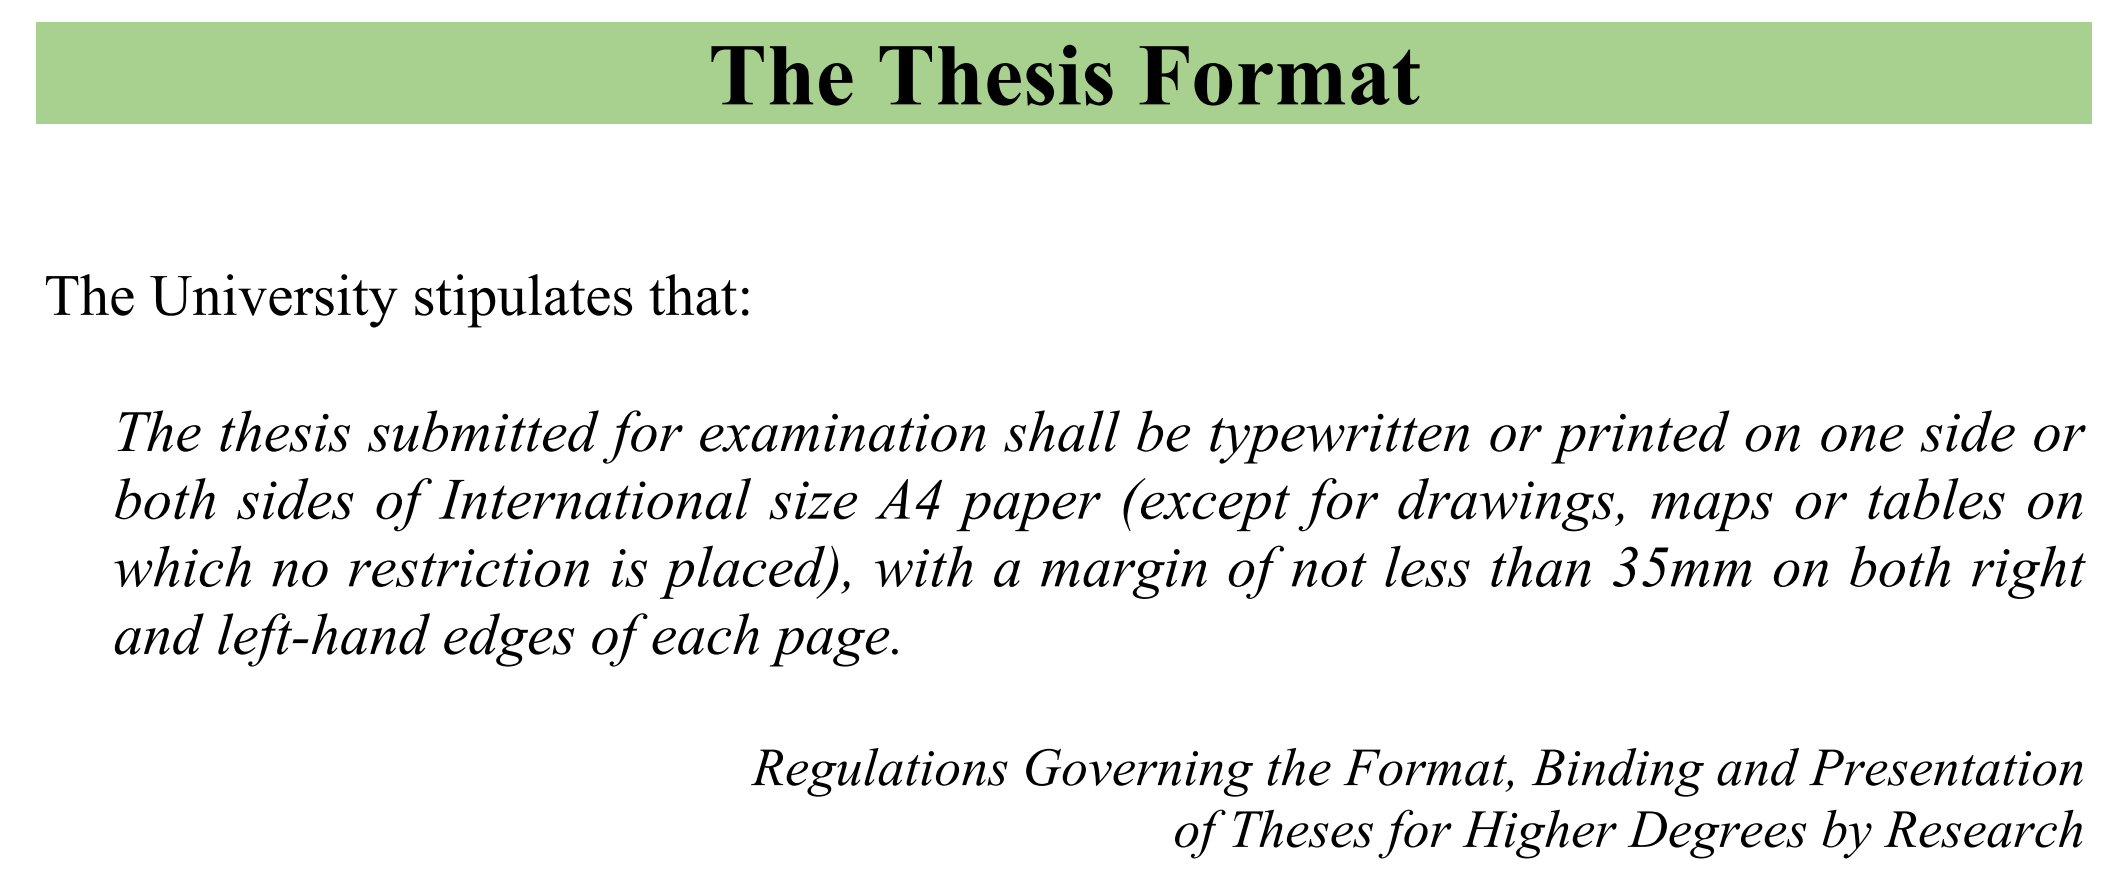
\includegraphics[width=.96\textwidth]{Figures/Chapter1/thesis_requirement.PNG}
%     \caption{Requirements of the thesis format in the Graduate School $13^\mathrm{th}$ edition booklet at Page 9.}
%     \label{fig:chap1:thesis_requirements}
% \end{figure}

% =========================================================== %
%                    Subsection: Astrocytes                   %
% =========================================================== %
\subsection{Astrocytes}
\label{chap1:sec:2:subsec1:astrocytes}
Astrocytes are the most abundant type of glial cell and represent up to $40\%$ of all the cells in the mammalian brain [Herculano-Houzel, 2014].
Despite being one of the first glial cells to be discovered around 150 years ago, their description and the understanding of their role in the brain function is far from complete.
As with everything in biology (is getting annoying really), astrocytes do not represent single homogeneous cell type and can be subdivided into several types depending on their morphology, molecular profile or function. 

From the morphological point of view astrocytes can be roughly divided into two types: \textbf{fibrous} and \textbf{protoplasmic}.
The first one is a star-shaped cell with regular contours present mainly in the white matter of the brain and spinal cord and in the optic nerve and the retina fiber layer.
Fibrous astrocytes are characterized by their elongated morphology, with long processes running parallel to the axon bundles that make contact with myelinated axons and with oligodendrocytes.
They have fewer processes compared to protoplasmic astrocytes.
Their processes spatially overlap in their domains and extend to perivascular, subpial and axonal endfeet [Lundgaard et al., 2014].

Protoplasmic astrocytes on the other hand have a “bushy” and irregular morphology, with a small round somata of $\sim 10 \mu m$ in diameter.
Present $5-10 \sim 50 \mu m$ primary processes, that further branch into thousands of branchlets and leaflets that form dense arborisations that connect with synapses [Bushong et al., 2002], and large endfeet that in turn connect with the vasculature [Nagelhus and Ottersen, 2013; Verkhratsky, Nedergaard and Hertz, 2015].
Unlike fibrous astrocytes, protoplasmic astrocytes populate mainly the gray matter in the brain and have domains with well defined borders that do not overlap between each other [Bushong et al., 2002].
Even when the the area of influence of an astrocyte is limited to local domains and do not mix with other astrocytes, it is highly connected and has a strong influence in neuronal activity.  
A single astrocyte arborisation can cover 20,000 to 80,000 $\mu m^3$, contacting 300 to 600 dendrites and potentially 100,000 individual synapses [Bushong et al., 2002, Halassa et al., 2007].
This dense connectivity allows astrocytes to control several processes like ion homeostasis or neurontransmitter recycling.
Interestingly, astrocytic domain boundaries have been proposed to be determined by, or at least closely relate to, neuronal functional units [Perea, Sur and Araque, 2014].
In this sense astrocytes could play the role of controlling and modulating \textit{functional islands} formed by the synapses confined within the area of influence of a single astrocyte [Halassa et al., 2007].
Further supports this hypothesis the fact that branching and connectivity of astrocyte, even from the same type, strongly depends on brain region.  
When comparing striatal and hippocampal astroglial populations it was noted that, despite having the same somatic volume, equivalent number of primary branches, and the same total cell volumes, hippocampal astrocyte territories are more constrained and display a tighter physical interaction with excitatory synapses [Chai et al., 2017] compare to striatal ones.

If astrocytes are so closely related to neuronal function and, as said before, have a big and dense areas of influence, what are astrocytes functions in the brain? 
This question represents still a very active area of research. Here we will enumerate some of the known functions that astrocytes fulfill but will later describe in more detail the role of astrocytes in modulating neuronal activity. 

Astrocytes are involved in the \textbf{control of cerebral blood flow} through \textbf{gliovascular coupling}.
Matching the blood flow to the neuronal metabolic needs is crucial for healthy brain functioning, this is achieved by astrocytes in a two-fold manner. 
First by regulating dilation of blood vessels: it has been proved that synaptic activity mediates cytoplasmic calcium increases in astrocytes, that in turn promote dilation of neighbouring arterioles [Zonta et al., 2003, Attwell et al., 2010].
At the same time, astrocytes regulate vasoconstriction through the release of 20-hydroxyeicosatetraenoic acid (20-HETE) [Zonta et al., 2003, Metea and Newman, 2006].
Interestingly, astrocytes seem to \textit{decide} weather to drive dilation or constriction based on local oxygen levels and metabolic states [Macvicar and Newman, 2015]. 

Given the enormous energy consumption in the brain, the regulation of oxygen and glucose availability must be tightly controlled.
This is, of course, in part regulated by blood flow. However, while oxygen freely diffuses in the brain, glucose and other metabolites need specialised transporters to travel through cell membranes.
The need for energy depends on neuronal activity, that can go from completely silent to high firing rate in miliseconds, which in turn can demand up to 30-fold increase in metabolic consumption [Attwell and Laughlin, 2001]. 
It has been demonstrated that astrocytes, who are in contact both with blood vessels and synapses, strongly and tightly control active \textbf{metabolic support} to neurons. 
This can be achieved through a variety of processes that are still an intense area of study. 
Glucose is preferentially taken by astrocytes rather than neurons [Pellerin et al., 2007], that enters glycolysis and produces lactate.
Lactate is then delivered to neurons via the astrocyte-neuron lactate shuttle (ANLS) [Pellerin and Magistretti, 1994)]. 
Meaning that astrocytes are not only involved in the metabolic support of neurons through blood flow regulation but also through direct delivery of energy substrates. 

Astrocytes, together with microglia, have a key role in the \textbf{immune response} of the brain, both in physiological and pathological conditions.
Upon brain injury or decease, astrocytes become reactive, drastically changing gene expression and entering full metal fight mode [Zamanian et al., 2012].
This changes induce morphological and functional alterations that lead astrocytes to enter one of two distinct reactivity profiles, depending on the nature of the insult. 
Inflammatory insult leads astrocytes to enter what has been called \textit{A1}, a reactivity profile implied in synapse pruning suggesting a detrimental role.
On the other hand, ischemic injury leads to activation of reactivity profile \textit{A2} responsible for growth and survival of neurons and synapses, indicating a protective role. 
Such contrasting mechanisms coexisting in the same cell type proves once more, the complexity, diversity and specificity of astrocytic function. 
Moreover, in physiological conditions, astrocytes continue to play a role in immune protection of the brain by maintaining the blood-brain barrier (BBB). 
Interestingly, astrocytes have been shown to be involved in BBB formation during development [Hayashi et al., 1997]. 

Besides the aforementioned functions, astrocytes play key roles in Ion [Sibille, Pannasch and Rouach, 2014, Nwaobi et al., 2016], water [Nielsen et al., 1997, Risher, Andrew and Kirov, 2009] and neurotransmitter [Danbolt, 2001, Herman and Jahr, 2007] homeostasis. 
Astrocytes can rapidly change their volume and intercellular communicative capacity, which allows them to redistribute water across astrocytic networks.  
Can redistribute $K^+$ ions through $K^+$ spatial buffering, and are the only cells in the central nervouse system that can synthesize glutamate and GABA from glucose. 
Astrocytes are an incredible versatile and complex cell that account for an incommensurate amount of functions and roles in the brain, however the aspect of astrocytes that concerns this work relates to the signaling in astrocytes and its relation with neuronal activity. 
We will discuss this aspects next. 
% =========================================================== %
%        Subsection: Calcium signaling in astrocytes          %
% =========================================================== %
\subsection{Calcium signaling in astrocytes}
\label{chap1:sec:2:subsec1:astro_calcium_signals}
As inexpert scientists, we PhD students have a bias view of the way research works towards positive discoveries and confirmed hypothesis. 
Simply because our biggest source of information are publications, and the chances of getting a story published that states "\textit{we formulated \textbf{this} hypothesis, and found it to be wrong}" are very low, there's a lack of charm in failure that prevents unsuccessful hypothesis to be known. 
Which is regrettable, because proven wrong hypothesis are at least as informative as positive results.
With brilliant examples like the Michelson-Morley experiment in 1887, where the two physicist trying to prove the existence of the aether, the medium in which light was thought to propagate, proved instead that it didn't exist.  
And in the way invented the interferometer. 
Invention that was later crucial for the development of the special theory of relativity and, more recently, for the detection of gravitational waves.
We can go even further and say that logic allow us \textit{only} to falsify theories, but, on the other hand, to prove a theory \textit{correct} is impossible. 
We can get encouraging results, experiments that help us gain confidence in our working hypothesis, but not really prove it.
On the other hand, one counterexample is all that is needed to prove it wrong.
As Einstein eloquently put it: \textit{The scientific theorist is not to be envied. For Nature, or more precisely experiment, is an inexorable and not very friendly judge of his work. It never says "Yes" to a theory. In the most favorable cases it says "Maybe," and in the great majority of cases simply "No." If an experiment agrees with a theory it means for the latter "Maybe," and if it does not agree it means "No." Probably every theory will someday experience its "No"—most theories, soon after conception.} [Albert Einstein: the human side: New glimpses from his archives. Dukas and Hoffman 1922]
Perhaps a way to compensate for this bias is to get rid of the miss-conception that falsifying an hypothesis represent failure but instead call it for what it is, a scientific discovery.  

In a way, a fruitful, but less interesting substitute of self-falsified hypothesis are the stories of scientist trying to prove \textit{other} peoples theories wrong, because controversy, unlike failure, sells journals.
One of the highly interesting and still active controversies in neuroscience is the question whether calcium concentration elevations in astrocytes regulates neuronal and vascular function.
This has led in the last few decades to a series of works by different groups that appeared to be contradictory, and different research lines have been seemingly proving each other wrong to give rise to a better and more profound understanding of the subject.  
We will not refer here the complete story that has been brilliantly summarized by Bazargani and Attwell [Bazargani and Attwell 2016], but will refer only some characteristics of calcium signaling in astrocytes that are relevant for the understanding of this work.

It's important to note first, that astrocytes, unlike neurons, are non-excitable cells.
For this reason, $Ca^{2+}$ fluctuations have been considered as the main intracellular readout of detection of environmental changes.
That includes astrocyte-neuron communication. 
An extensive amount of work in the last few decades has been dedicated to understand the origin of $Ca^{2+}$ transients, if this fluctuations are somehow relevant for neuronal regulation, and if so, how.
To the date most of this questions remain unanswered, although currently there seems to be a common consensus in the field that (spoiler alert) they are at least involved in several regulation pathways, and respond, in physiological conditions to behavioral and sensory correlates. 

Should caught our attention the fact that baseline levels of $Ca^{2+}$ in astrocytes are higher than that of neurons, and that this concentration vary inside each cell, being higher in processes compared to the soma [Zheng et al., 2015].
Which already suggest two observations: first, the relevance of $Ca^{2+}$ in astrocytic signaling, and second, the within-cell complexity of it. 
In astrocytes, $Ca^{2+}$ fluctuations can have different sources, the first of which is intrinsic. 
In fact, it was shown that $65\%$ of astrocytes in hippocampal slices exhibit asynchronous and localised $Ca^{2+}$ transients, even in the absence of neuronal activity [Nett et al., 2002].
The role and relevance of these untriggered events has yet to be defined. 
Specially because it's unclear if this spontaneous events do happen in physiological conditions and if so, in which fashion. 

More interesting are \textbf{$Ca^{2+}$ changes induced by neuronal activity}.
Glutamate has been shown to evoke calcium concentration rise in astrocytes in several contexts, in culture [Cornell-Bell et al., 1990], in brain slices [J.W. Dani et al., 1992], in whole retina [Newman and Zahs 1997] and \textit{in vivo} [Wang et al. 2006].
This calcium transients can propagate along astrocyte processes and even between glial cells [ornell-Bell et al., 1990, J.W. Dani et al., 1992, Hirase, H. et al., 2004, Nimmerjahn, A. et al., 2004].
This observations further support the possibility that glial Ca2+ waves might constitute an extra-neuronal signaling system in the CNS, and, importantly, that it can be driven by neuronal activity. 
However, to begin to understand the neuron-astrocytic $Ca^{2+}$ activity relation one must realize that, just like neurons, astrocytes have to be thought as the sum of many different subcellular compartments and that calcium transients occurring in the soma are very different and can have different sources as the the ones in fine astrocytic processes near synapses.
$Ca^{2+}$ events in processes can occur independently of larger ones in the soma, which suggest that regulation of synapses or blood vessels can happen locally. 
This events can, however, propagate to neighbouring intracellular areas [Di Castro et al., 2011] or even synchronise with neighbouring cells [Takata et al., 2013].
Importantly, it has been shown that such events correlate with the strength of neuronal activity [Panatier et al., 2011].

Process and soma $Ca^{2+}$ events also differ in their temporal profile.
While is true that somatic calcium transients are several order of magnitude longer than neuronal action potentials, which has been an historical argument against the hypothesis that astrocyte could be involved in real-time information processing in the brain, smaller events occur in processes even in the subsecond scale [Winship, Plaa and Murphy, 2007; Lind et al., 2013, 2018].
This partially solves the temporal argument, but in a more fundamental aspect, it's by no means clear if information processing in neuronal network relies in temporal or rate coding or a combination of both.
Rate coding responses could be an alternative way in which long lasting astrocytic $Ca^{2+}$ signals could be involved in a relevant temporal scale in neuronal activity and information processing [Semyanov, 2019].
On a further bigger scale, $Ca^{2+}$ events can propagate as waves through networks of several tens and even hundreds of astrocytes.
Behavior that  has been observed in cultures [Cornell-Bell et al., 1990b], as well as \textit{in vivo} in the frontal and parietal cortices upon sensory stimulation []Ding et al., 2013] and in the cerebellum during locomotion [Nimmerjahn, Mukamel and Schnitzer, 2009].
Giving rise to the possibility of astrocytes modulating neuronal activity at a network scale. 

As stated before, many of such calcium transients have been shown to depend, or have its origin in neuronal activity dependent processes. 
In hippocampal dentate gyrus astrocytes action potential–driven synaptic transmitter release triggers large and long lasting ($\sim3 s$), spatially broad ($\sim12 \mu m$) events, while spontaneous synaptic transmitter release produces brief ($\sim 0.7 s$), spatially localized ($\sim 4 \mu m$) transients [Di Castro, M.A. 2011].
It has been suggested that release of $Ca^{2+}$ from internal stores could be the main source of $Ca^{2+}$ somatic transients, while in the astrocyte processes transmembrane entry of Ca2+, presumably through endogenously active channels such as TRPA1 [Shigetomi, 2012] or receptor-gated $Ca^{2+}$-permeable ion channels, generates 30–40\% of $Ca^{2+}$ concentration elevations. 
In this way while $Ca^{2+}$ rises in astrocyte somata may be too slow [Schummers, et al. 2008, Schulz, K. et al, 2012] to generate rapid blood flow increases, $Ca^{2+}$ transients in the processes that are faster than in the soma [Tang, W. et al. 2015] occur before or with a similar time course to the increase of blood flow [Lind, B.L. 2013, Otsu, Y. et al, 2015].

We will not dig into the specific mechanisms through which neuronal activity could induce such calcium transients (related to the activation of mGluR receptors by glutamate release) or the controversies involved. 
But will instead mention some of the observations that evidence astroctytic calcium transients physiological relevance. 
It has been observed that whisker stimulation increases $Ca^{2+}$ concentration in astrocytic cytoplasm in the barrel cortex [Wang et al., 2006], in a frequency dependent manner [Perea and Araque, 2005; Sherwood et al., 2017]. Other behavioural variables like locomotion or arousal state have been observed to evoke $Ca^{2+}$ elevation over broad spatial areas, mediated by noradrenaline signals in the frontal and parietal cortex [Ding et al., 2013, Paukert, et al., 2014].
Suggesting an astrocytic involvement in the control and modulation of sensory input and behavior. 

The complexity both in source and dynamical properties of calcium oscillations in astrocytes makes it rather complicated but at the same time extremely interesting to study.
Astrocyte calcium changes are related to neuronal activity, to neurotransmitter release and to sensory input and behavioral state.
Can occur in fast transients in the processes or in longer, stronger events in the soma. 
Can propagate within the cell, across neighbouring cells and through extended networks.
But what is the role (or roles), if any, of each of this astrocytic calcium dynamics in the processing of information by neuronal networks? We will summarize some of recent results regarding this question in the following section.

% =========================================================== %
%   Subsection: Astrocityc modulation of neuronal activity    %
% =========================================================== %
\subsection{Astrocityc modulation of neuronal activity}
\label{chap1:sec:2:subsec2:astro_neuromodulation}

So far we have been dealing with how astrocytes can be involve the way in which neurons process information, but a parallel and relevant question is if and how astrocytes process information themselves. 
% =========================================================== %
%        Subsection: Astrocytes accumulate evidence           %
% =========================================================== %
\subsection{Astrocytes accumulate evidence}
\label{chap1:sec:2:subsec4:astro_evidence}
Refer to paper from \textit{Misha Harens}

% ================================================================ %
% Section: Astrocytes encode spatial information in Ca2+ activity  %
% ================================================================ %
\section{Astrocytes encode spatial information in $Ca^{2+}$ activity}
\label{chap1:sec3:astro_spat_info}

% =========================================================== %
%        Subsection: Astrocytes and information               %
% =========================================================== %
\subsection{Astrocytes and information}
\label{chap1:sec:3:subsec1:astro_info}
Treating astrocytes $Ca^{2+}$ activity with Information theory approaches

% =========================================================== %
%             Subsection: Decoding of position                %
% =========================================================== %
\subsection{Decoding of position}
\label{chap1:sec:3:subsec2:position_decoding}

% =========================================================== %
%                    Subsection: Page Margin                  %
% =========================================================== %
% \subsection{Page Margin}
% \label{chap1:sec:2:subsec1:page_margin}
% The format of page size and margin is defined in ``main.tex'' file \textbf{Line 63-71}. The page margin of the current version template is \uline{Left: 35mm, Right: 36mm (a4paper).} Users can change the page margin by adjusting the corresponding settings. There is no stipulation for the top and bottom margins, but the booklet recommend that both of them should be 25mm, which is adopted in this template. 


% =========================================================== %
%          Subsection: Font, Alignment, Line Spacing          %
% =========================================================== %
% \subsection{Font, Alignment, Line Spacing}
% Ordinarily, there is no restrict stipulation for the font family, font size, alignment, and line spacing. All of these are a matter of personal preference. This template uses \textit{10pt} font size, \textit{Fully Justified} alignment style and \textit{One and A Half} line spacing. Users can adjust the settings in \textbf{Line 19-33} of the ``main.tex'' file to change the typeset.


% =========================================================== %
%                      Subsection: Contents                   %
% =========================================================== %
% \subsection{Contents}
% The contents of this template can be subdivided into three parts --- the front matter, the text and the back matter, which strictly follows the stipulations of the official booklet (Page 17). \tabref{chap1:longtable:checking_list} indicates the what contents are required in the submitted thesis and what contents are optional. The column ``Required'' denotes that 
% \begin{center}
% \begin{longtable}{|l|c|c|}
% \caption{Checking list indicating the contents should be included in the thesis.}\label{chap1:longtable:checking_list}\\
% \hline
% \textbf{The Front Matter} & Required     &  Include $\checkmark$ \\ \hline \hline
% Abstract                  & Yes          & $\checkmark$         \\
% Title Page                & Yes          & $\checkmark$         \\
% Frontispiece              &              &                      \\
% Dedication                &              & $\checkmark$         \\
% Epigraph                  &              &                      \\
% Declarations              & Yes          & $\checkmark$         \\
% Acknowledgements          &              & $\checkmark$         \\
% Table of Contents         & Yes          & $\checkmark$         \\
% List of Illustrations     &              &                      \\
% List of Figures           &              & $\checkmark$         \\
% List of Tables            &              & $\checkmark$         \\
% List of Algorithm         &              & $\checkmark$         \\
% List of Abbreviations     &              & $\checkmark$         \\
% List of Symbols           &              & $\checkmark$         \\
% Others                    &              &                      \\ \hline \hline
% \textbf{The Text}         & Yes          & $\checkmark$         \\ \hline \hline
% \textbf{The Reference or Back Matter} &    ---    &   ---       \\ \hline \hline
% Glossary                  &              &                      \\
% Appendices                &              &                      \\
% Notes                     &              &                      \\
% Bibliography or Reference List & Yes          &  $\checkmark$   \\
% Index                     &              &                      \\
% \hline
% \end{longtable}
% \end{center}
% This template support most of the contents listed in the figure, including the ``Abstract'', ``Title Page'', ``Declarations'', ``Acknowledgements'', ``List of Publications'', ``Contents'', ``List of Figures'', ``List of Tables'', ``List of Algorithms'', ``List of Abbreviations'', ``List of Symbols'', ``Main Text'', ``Appendices'', and ``Bibliography''. Each part is defined in an independent tex file and the ``main.tex'' file combines all the different parts to form the entire thesis. Therefore, users can easily make the changes by adjusting the corresponding document files.

% In addition to the stipulations of the booklet, this template also provides a beautiful \textbf{cover page}, which is the first two pages of this project. \uline{The cover page is \textbf{not required} by the Graduate School and you'd better remove the cover page when bounding your thesis for submission.}








